\subsection{Aufbau der Messapparatur}
%
%- Spektrallampe\\
%- Sammelline/Kollimator\\
%- $D_{1}$-Interferenzfilter\\
%- Polarisationsfilter + $\lambda/4$-Platte\\
%- Dampfzelle\\
%  --- Heizer\\
%- Helmholtzspulenpaare\\
%  --- Vertikalfeld\\
%  --- Horizontalfeld\\
%  --- Sweepfeld\\
%  --- RF-Feld mit Frequenzgenerator (Sinusspannung)\\
%- Kollimator\\
%- Photodetektor\\
%- Verstärker\\
%- Oszilloskop\\
%
\begin{figure}[h!]
  \centering
  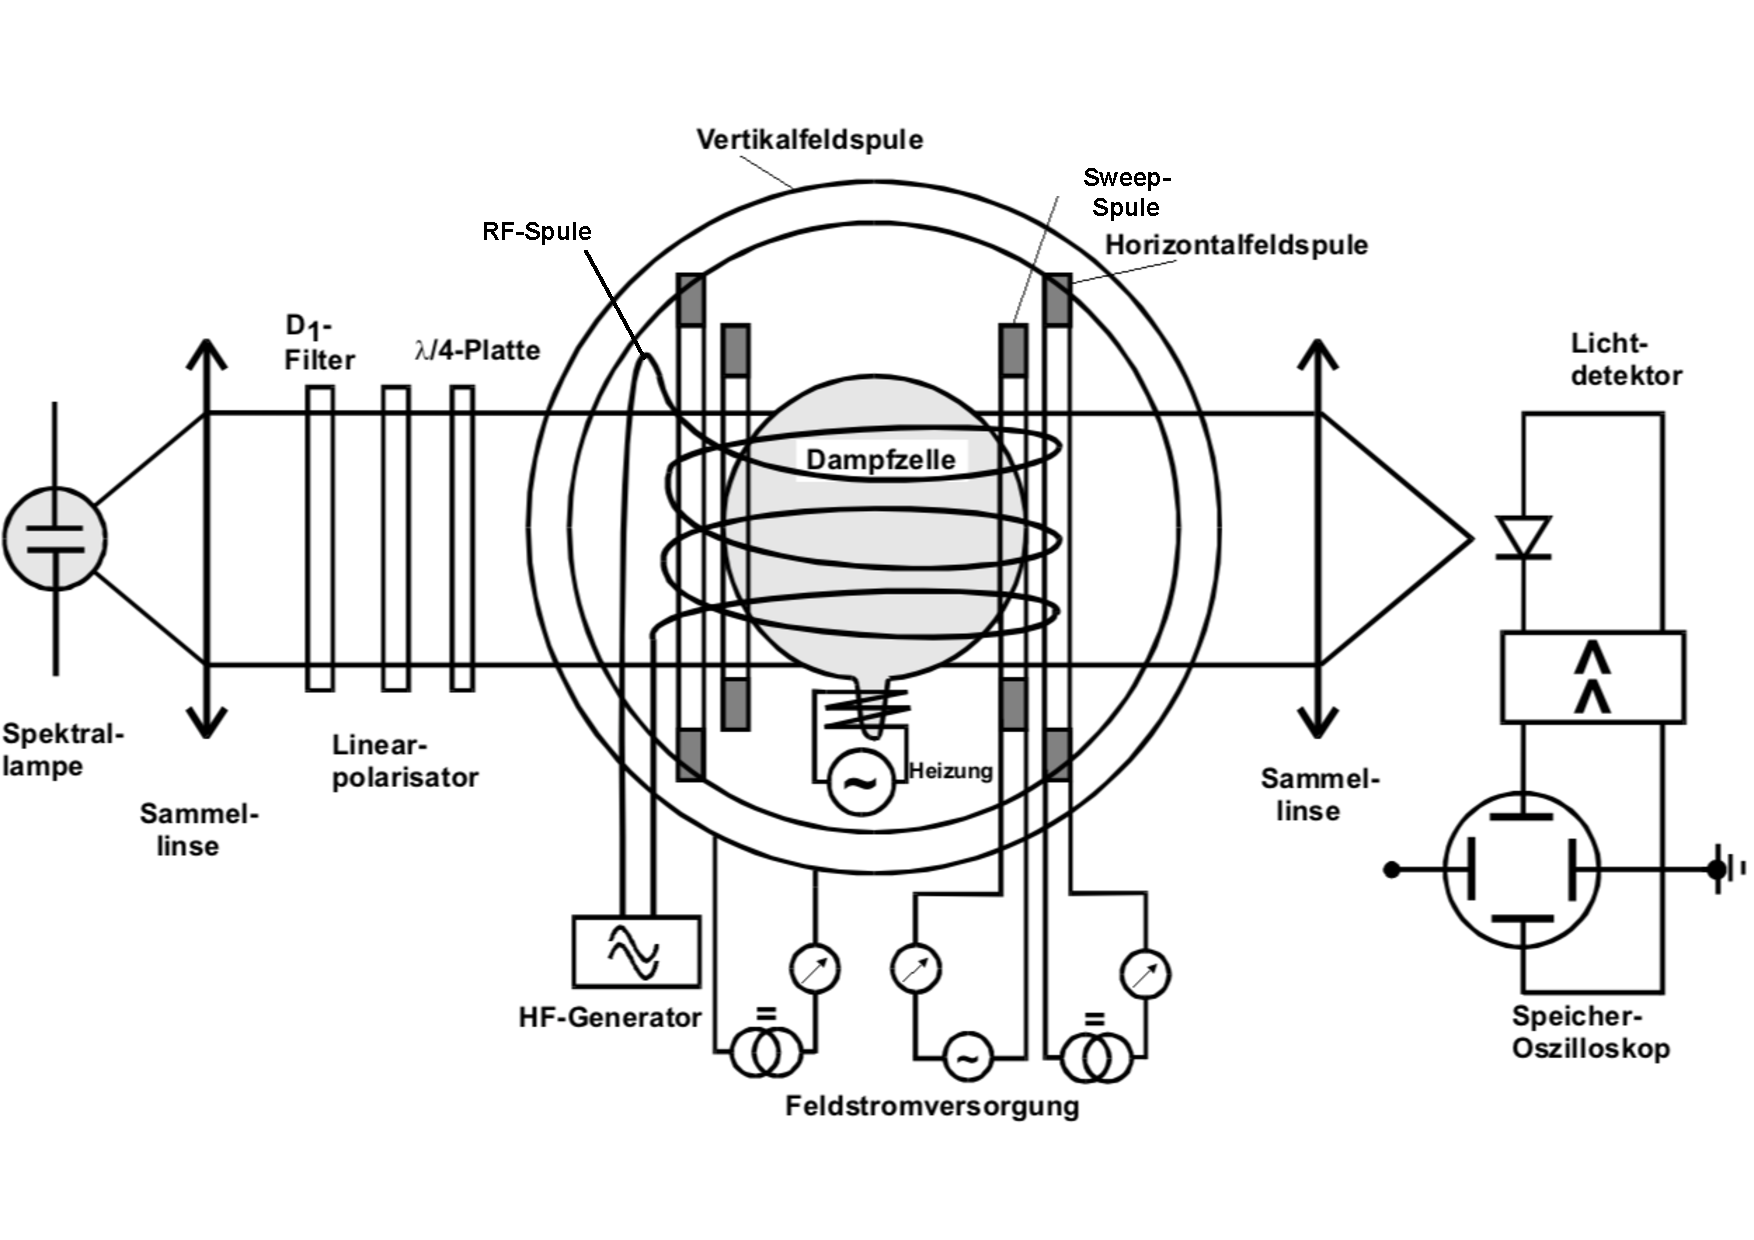
\includegraphics[width=\textwidth]{aufbau.pdf}
  \caption{Schematischer Aufbau der Messapparatur \cite{1}, bearbeitet}
  \label{fig:aufbau}
\end{figure}
Der Aufbau setzt sich zusammen aus einer Spektrallampe, einem Kollimator (Sammellinse), einem $D_{1}$-Interferenzfilter, einem Polarisationsfilter und $\lambda/4$-Platte, der Dampfzelle mit Heizer, vier Helmholtzspulenpaaren, ein Kontrollgerät für die Stärke der Magnetfelder, einem weiteren Kollimator, einen Photodetektor, einem Verstärker und einem Oszilloskop.
\\Die Spektrallampe gibt das Rubidium-Spektrum aus, der Kollimator parallelisiert die Strahlen.
Der $D_{1}$-Interferenzfilter lässt nur das $D_{1}$-Licht passieren.
Der Polarisationsfilter und die $\lambda/4$-Platte polarisieren das $D_{1}$-Licht zu $\sigma^{+}$-Licht.
In der Dampfzelle befinden sich zwei Rubidium-Isotope, $^{85}Rb$ und $^{87}Rb$, die mit dem Heizer verdampft werden.
Die vier Helmholtzspulenpaare bilden die Vertikalfeldspule, die Horizontalfeldspule, die Sweepspule und die RF-Spule, welche von einem Hochfrequenz-Generator mit einer Sinusspannung gespeist wird.
Die anderen drei Spulen werden über das Kontrollgerät angesteuert.
Mithilfe dreier Potentiometer lässt sich der Strom durch die Spulen einstellen.
Das Vertikalfeld wird dazu genutzt, um die vertikale Komponente des Erdmagnetfelds zu kompensieren.
Mit dem Horizontalfeld und dem Sweep-Feld wird das äußere Magnetfeld der Apparatur verändert, um die Resonanzstellen zu angelegten Frequenz des RF-Felds zu finden.
Mit der RF-Spule und der angelegten hochfrequenten Sinusspannung wird das RF-Feld erzeugt, welches zur induzierten Emission und damit zu den Resonanzstellen führt.
Der zweite Kollimator bündelt das Licht auf den Photodetektor.
Der Photodetektor misst die eintreffende Intensität und gibt sie als Spannung aus.
Die Photodetektorspannung wird mithilfe des Oszilloskops nach vorheriger Verstärkung dargestellt und ausgemessen.

\subsection{Vorbereitung}
%
%- Intensitätsmaximum der optischen Elemente auf den Photodetektor bringen\\
%- Ausrichten des Tisches mit der Messapparatur\\
%- Vertikalfeld erhöhen bis der Peak auf dem Oszilloskop möglichst schmal ist\\
%
Zur Vorbereitung werden die optischen Elemente auf der optischen Bank so ausgerichtet, dass das Intensitätsmaximum auf dem Photodetektor liegt.
Anschließend wird der Tisch und die sich darauf befindende Apparatur mithilfe eines Kompasses so weit gedreht, bis der Tisch parallel bzw. antiparallel zur horizontalen Komponente des Erdmagnetfelds steht.
Auf dem oszilloskop ist ein breiter, nach oben geöffneter Peak zu sehen, der mit der Anpassung des Vertikalfeldes schmaler wird.
Das Vertikalfeld wird so eingestellt, dass der Peak möglichst schmal ist.
Damit sind alle Vorbereitungen getroffen.

\subsection{Messung der Resonanzstellen}
%- RF-Frequenz setzen ($\nu=\SI{100}{}-{1000}{kHz}$)\\
%- B-Feld der Sweep-Spule erhöhen, um Resonanzstelle des B-Felds zu finden\\
%- B-Feld propotional zu den Umdrehungen des verwendeten Potentiometers, Strom durch Potentiometerumdrehungen ablesen\\
%- Horizontalfeld ebenfalls erhöhen um Resonanzstellen ins Bild des Oszilloskop zu bringen\\
%- Frequenz, Umdrehung Sweep-Spule für beide Isotope, Umdrehung Horizontalfeldspule für beide Isotope notieren\\
%
Die Messung der Resonanzstellen beginnt, indem an der RF-Spule eine Frequenz von $\nu=\SI{100}{}-{1000}{kHz}$ anlegt wird.
Anschließend wird das Sweepfeld durch Drehen am dazugehörigen Potentiometer erhöht.
Die Magnetfelder der Spulen sind direkt abhängig von den Umdrehungen an den Potentiometern.
Mithilfe des Oszilloskops wird die Darstellung des Messpunktes mit der Nachleuchtzeit so gewählt, dass die Resonanzstelle mit dem Potentiometer ausgemessen werden kann.
Ab der zweiten Frequenz reicht der Bildausschnitt des Oszilloskops nicht aus, um die Resonanzstelle zu zeigen.
Daher wird das Horizontalfeld erhöht, bis die Resonanzstelle im Bild ist.
Dann wird das Sweepfeld nach obiger Angabe erhöht.
Es werden $10$ verschiedene Frequenzen zwischen $\nu=\SI{100}{}-{1000}{kHz}$ an die RF-Spule gelegt.
%
